\documentclass{article}

\usepackage{polski}
\usepackage[utf8]{inputenc}
\usepackage{booktabs}
\usepackage{biblatex}
\usepackage{subfigure}
\usepackage{graphicx}
\usepackage{float}
\usepackage{geometry}
\usepackage{listings}

 \usepackage[table,xcdraw]{xcolor}

\geometry{
	a4paper,
	total={170mm,257mm},
	left=50mm,
	right=50mm,
	top=45mm,
	bottom = 45mm
}
\usepackage{tabularx}


\begin{document}
	\newgeometry{tmargin=4cm, bmargin=4cm, lmargin=3cm, rmargin=3cm}
	
	\begin{titlepage}
		\center
		\newcommand{\HRule}{\rule{\linewidth}{0.6mm}}
		
		\textsc{\LARGE Politechnika Wrocławska}\\[1.5cm]
		\textsc{\Large Laboratorium}\\[0.5cm] 
		\textsc{\large Inteligencja Obliczeniowa i jej Zastosowania}\\[0.7cm] 

		\HRule \\[0.4cm]
		{ \huge \bfseries Algorytmy ewolucyjne i hybrydowe}\\[0.4cm]
		\HRule \\[1.5cm]
		
		\begin{minipage}{0.4\textwidth}
			\begin{flushleft} \large
				\emph{Authors:}\\
				Rafał \textsc{Pieniążek}\\
                Jakub \textsc{Pomykała}
			\end{flushleft}
		\end{minipage}
		~
		\begin{minipage}{0.4\textwidth}
			\begin{flushright} \large
				\emph{Supervisor:} \\
				prof. dr inż. Olgierd \textsc{Unold} 
			\end{flushright}
		\end{minipage}\\[4cm]

		{\large \today}\\[3cm]
		
		\vfill
		
	\end{titlepage}
\tableofcontents
\newpage
\listoffigures
\newpage
\section{Wstęp}
	Celem laboratorium było przeprowadzenie optymalizacji globalnej dla wybranych funkcji z pakietu globalOptTests.
    

\section{Zastosowany algorytm optymalizacji}

W laboratorium zastosowano algorytmy genetyczne będące klasą algorytmów ewolucyjnych.
Algorytmy ewolucyjne stanowią kierunek sztucznej inteligencji, która wykorzystuje i symuluje ewolucję biologiczną. Wszystkie algorytmy tej klasy symulują podstawowe zachowania w teorii ewolucji biologicznej - procesy selekcji, mutacji i reprodukcji. Zachowanie jednostek zależy od środowiska. Zbiór jednostek nazywa się populacją. Taka populacja ewoluuje zgodnie z regułami selekcji zgodnie z funkcją celu przypisaną do środowiska. Propagowane do kolejnych pokoleń są tylko najbardziej dopasowane osobniki.


\subsection{Modyfikowane parametry}

W celu badania wpływu zmiennych na zachowanie algorytmu genetycznego modyfikowano następujące parametry:

\begin{itemize}
\item \textbf{elitarność} - Procentowa wartość populacji, która zostaje przeniesiona do następnego pokolenia bez zmian. Niezerowa wartość gwarantuje, że jakość rozwiązania nie zmniejszy się z pokolenia na pokolenie.

\item \textbf{mutacja} - Przypadkowa zmiana genomu w algorytmie genetycznym, analogicznie do mutacji biologicznej.

\item \textbf{krzyżowanie} -  Połączenie niektórych (wybranych losowo) genotypów w jeden. Kojarzenie ma sprawić, że potomek dwóch osobników rodzicielskich ma zespół cech, który jest kombinacją ich cech (może się zdarzyć, że tych najlepszych).

\item \textbf{liczba iteracji} - Ilość pokoleń  
\item \textbf{rozmiar populacji} - Ilość osobników w jednym pokoleniu.
\end{itemize}


\begin{table}[!htbp]
\centering
\caption{Wartości modyfikowanych parametrów}
\label{my-label}
\begin{tabular}{|l|l|}
\hline
\rowcolor[HTML]{C0C0C0} 
\textbf{Parametr}      & \textbf{Wartości}      \\ \hline
populacja              & 50, 100, 150, 200, 250 \\ \hline
liczba iteracji        & 50, 100, 150, 200, 250 \\ \hline
p. krzyżowania         & 0, 0.25, 0.5, 0.75, 1  \\ \hline
p. mutacji             & 0, 0.25, 0.5, 0.75, 1  \\ \hline
p. populacji elitarnej & 0, 0.25, 0.5, 0.75, 1  \\ \hline
\end{tabular}
\end{table}


\subsection{Zastosowane narzędzia implementacji}

\subsubsection{Język R}
R jest językiem programowania i środowiskiem programistycznym, używanym głównie do obliczeń statystycznych i wizualizacji danych, do sztucznej inteligencji a także do ekonomii i innych zagadnień wykorzystujących obliczenia numeryczne. Został stworzony przez Rossa Ihakę i Roberta Gentlemana na Uniwersytecie w Auckland w Nowej Zelandii. 


\subsubsection{Pakiet GA}

Pakiet GA zawiera zestaw funkcji ogólnego przeznaczenia do optymalizacji z wykorzystaniem algorytmów genetycznych. Dostępnych jest kilka operatorów genetycznych, których można łączyć w celu zbadania najlepszych ustawień dla bieżącego zadania.


\subsubsection{Pakiet globalOpts}
Pakiet zawierający implementację funkcji przydatnych do przeprowadzania testów wydajnościowych algorytmów optymalizacji globalnej.


\clearpage
\section{Funkcja Shuberta}
	\subsection{Wzór analityczny}
	   \begin{figure}[!htbp]
    \centering
    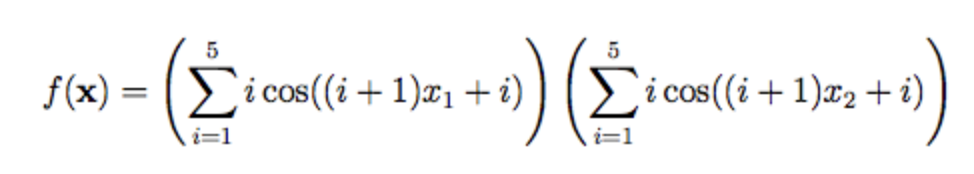
\includegraphics[width=0.6\textwidth]{inc/wzory/schubert}
     \caption{Wzór analityczny funkcji Schuberta}
    \end{figure}
    
    
 
    
    
    \subsection{Wykres w ustalonym przedziale zmiennych}
    
    \begin{figure}[!h]
    \centering
    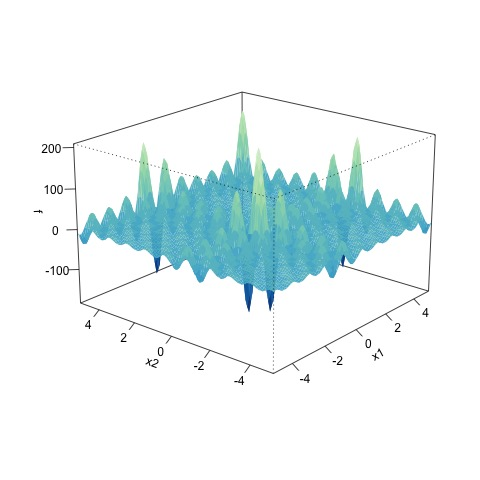
\includegraphics[width=0.6\textwidth]{inc/wykresyfunkcji/schubert}
     \caption{Wykres  funkcji Schuberta}
    \end{figure}
    
    \subsection{Ekstremum globalne}
    
       \begin{figure}[!h]
    \centering
    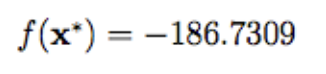
\includegraphics[width=0.3\textwidth]{inc/wzory/schubert-global-minimum}
     \caption{Minimum globalne dla funkcji Schuberta}
    \end{figure}
    
       \begin{figure}[!h]
    \centering
    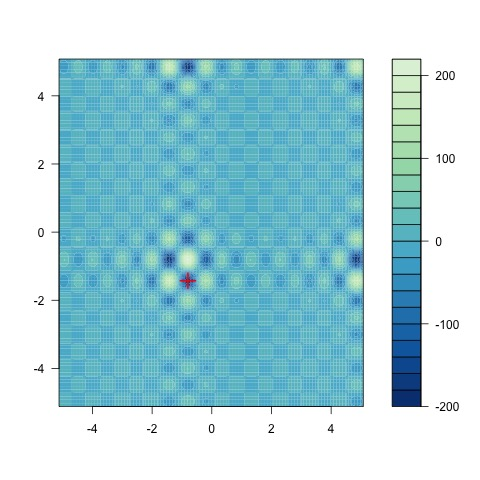
\includegraphics[width=0.7\textwidth]{inc/wykresyfunkcji/schubert-global-minimum}
     \caption{Minimum globalne dla funkcji Schuberta}
    \end{figure}
    
\subsection{Własne operatory krzyżowania i mutacji}
    
\subsubsection{Zmiana funkcji mutowania}
     \clearpage\begin{figure}[!htbp]
    \centering
    \mbox{
    \subfigure{
    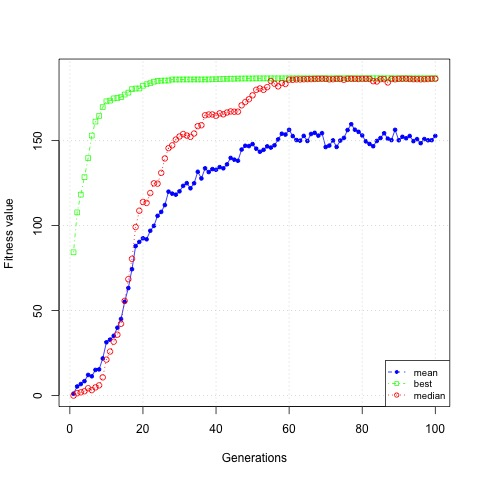
\includegraphics[width=3in]{{{inc/results/default_ga}}}\quad
    }
    \subfigure{
    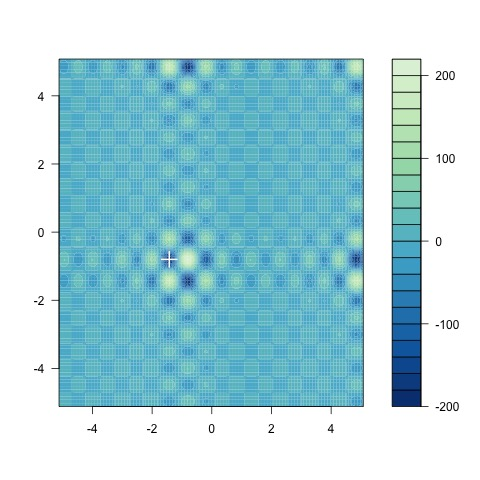
\includegraphics[width=3in]{{{inc/results/default_ga_result}}\quad
    }
    }
    \caption{Test optymalizacji GA Schubert p50 i100 c0.8 m0.1 e0.05}
    \end{figure}

\subsubsection{Zmiana funkcji krzyżowania}

                 


\section{Wnioski}

Badanie wpływu paramterów na jakość rozwiązań optymalnych poszukiwanych przez algorytm genetyczny jest zadaniem nietrywialnym, ale możliwym do wykonania. Zastosowanie pakietu GA dla języka R pozwoliło skupić się bardziej na testowaniu parametrów, a nie na implementacji algorytmu.

Warto zauważyć, że na jakość rozwiązań ma wpływ nie tylko wartość parametru, ale również funkcja poddawana testom. Dla tych samych zestawów danych wykresy testów różnią się pomiędzy testowanymi funkcjami. W przypadku poszukiwania ekstremum globalnego dla funkcji z wieloma ekstremami lokalnymi i  niekorzystnym doborze parametrów  algorytm  może nie znaleźć poprawnego rozwiązania. Jest to spowodowane stochastycznym doborem populacji początkowej.



\section{Literatura}
\begin{enumerate}
\item Artur Suchwałko, "Wprowadzenie do R dla programistow innych jezykow", \url{https://cran.r-project.org/doc/contrib/R-dla-programistow-innych-jezykow.pdf}, 2014-02-23
\item Luca Scrucca, "On some extensions to GA package:
hybrid optimisation, parallelisation and islands evolution", \url{https://arxiv.org/pdf/1605.01931.pdf}, 2016-05-09
\item dr inż. Julian Sienkiewicz, "Pakiet R w analizie układów złożonych", \url{http://www.if.pw.edu.pl/~julas/CSAR/csar11.html}, 2017
\item W. N. Venables, D. M. Smith, R Core Team, "An Introduction to R", \url{https://cran.r-project.org/doc/manuals/r-release/R-intro.pdf}, 2018-04-23
\item Luca Scrucca, "Package 'GA'", \url{ftp://cran.r-project.org/pub/R/web/packages/GA/GA.pdf}, 2016-09-29
\item Katharine Mullen, "Package 'globalOptTests'", \url{https://cran.r-project.org/web/packages/globalOptTests/globalOptTests.pdf},
2015-02-15
\item Abdal-Rahman Hedar, "Global Optimization Test Problems", \url{http://www-optima.amp.i.kyoto-u.ac.jp/member/student/hedar/Hedar_files/TestGO.htm}, dostęp online: 2018-05-04
\end{enumerate}

\section{Kod źródłowy}

%\lstset{
   % language=R,   
   % extendedchars=true,
  %  inputencoding=latin1,
%     basicstyle=\small
%}

%\lstinputlisting{inc/main.r}




\end{document}\documentclass{article}
